\documentclass{exam}
\usepackage{amsmath}
\usepackage{graphicx}
\def\myhrule{\vspace*{0.05in}\lower1ex\null\vadjust{\hrule}}

\pagestyle{head}
\header{\textit{\large Scripps Ranch High Physics Club}}{}{\thepage}
\firstpageheader{\textit{\large Scripps Ranch High Physics Club\myhrule}}{}{\large September 15, 2025 \myhrule}
\begin{document}
    \vspace*{-25px}
    \begin{center}
        \huge \textbf{Lagrangian Mechanics Problem Set}
    \end{center}
    \vspace*{0.05in}
    \Huge
    \begin{center}
        $\frac{\partial L}{\partial q}-\frac{d}{dt}(\frac{\partial L}{\partial \dot{q}})=0$
    \end{center}
    \begin{questions}
        \large
        \question Compute the following partial derivatives
        \begin{parts}
            \part $\frac{\partial}{\partial x} \, y\ln(x^2)-xw^2+e^w$
            \part $\frac{\partial}{\partial y} \, y\ln(x^2)-xw^2+e^w$
            \part $\frac{\partial}{\partial x} \, \cos(xy)+y^2$
            \part $\frac{\partial}{\partial x} \, y^x+x^y$
            \part $\frac{\partial}{\partial y} \, \cos(\sqrt{x^\pi})-\ln(x!)$
            \part $\frac{\partial}{\partial x} \, \sqrt{x+y}$
        \end{parts}
        \question In Figure 1 we show a box of mass $m$ sliding down a ramp of mass $M$. The ramp moves
without friction on the horizontal plane and is located by coordinate $x_1$. The box also slides without friction
on the ramp and is located by coordinate $x_2$ with respect to the ramp. Find $\ddot{x}_1$
        \begin{center}
            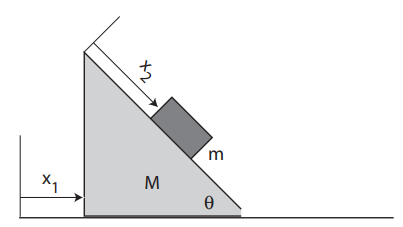
\includegraphics{../assets/figure1.png}\\
            Figure 1
        \end{center}\vspace{2in}
        \question A particle is subjected to the potential $V(x) = -Fx$, where F is a constant. The
particle travels from $x = 0$ to $x = a$ in a time interval $t_0$. Assume the motion of the
particle can be expressed in the form $x(t) = A + Bt + Ct^2$. Find the values of $A, B,$
and $C$ such that the action is a minimum. \vspace{2in}
        \question A pendulum of length $\ell_2$ and mass $m_2$ is strung to the bob of another pendulum of length $\ell_1$ and mass $m_1$. Use lagrangian mechanics to devise a set of formulas that describe the motion of this system (you will not be able to find a formula for $\theta_1$ and $\theta_2$. Don't worry, just go as far as you can)
        \begin{center}
            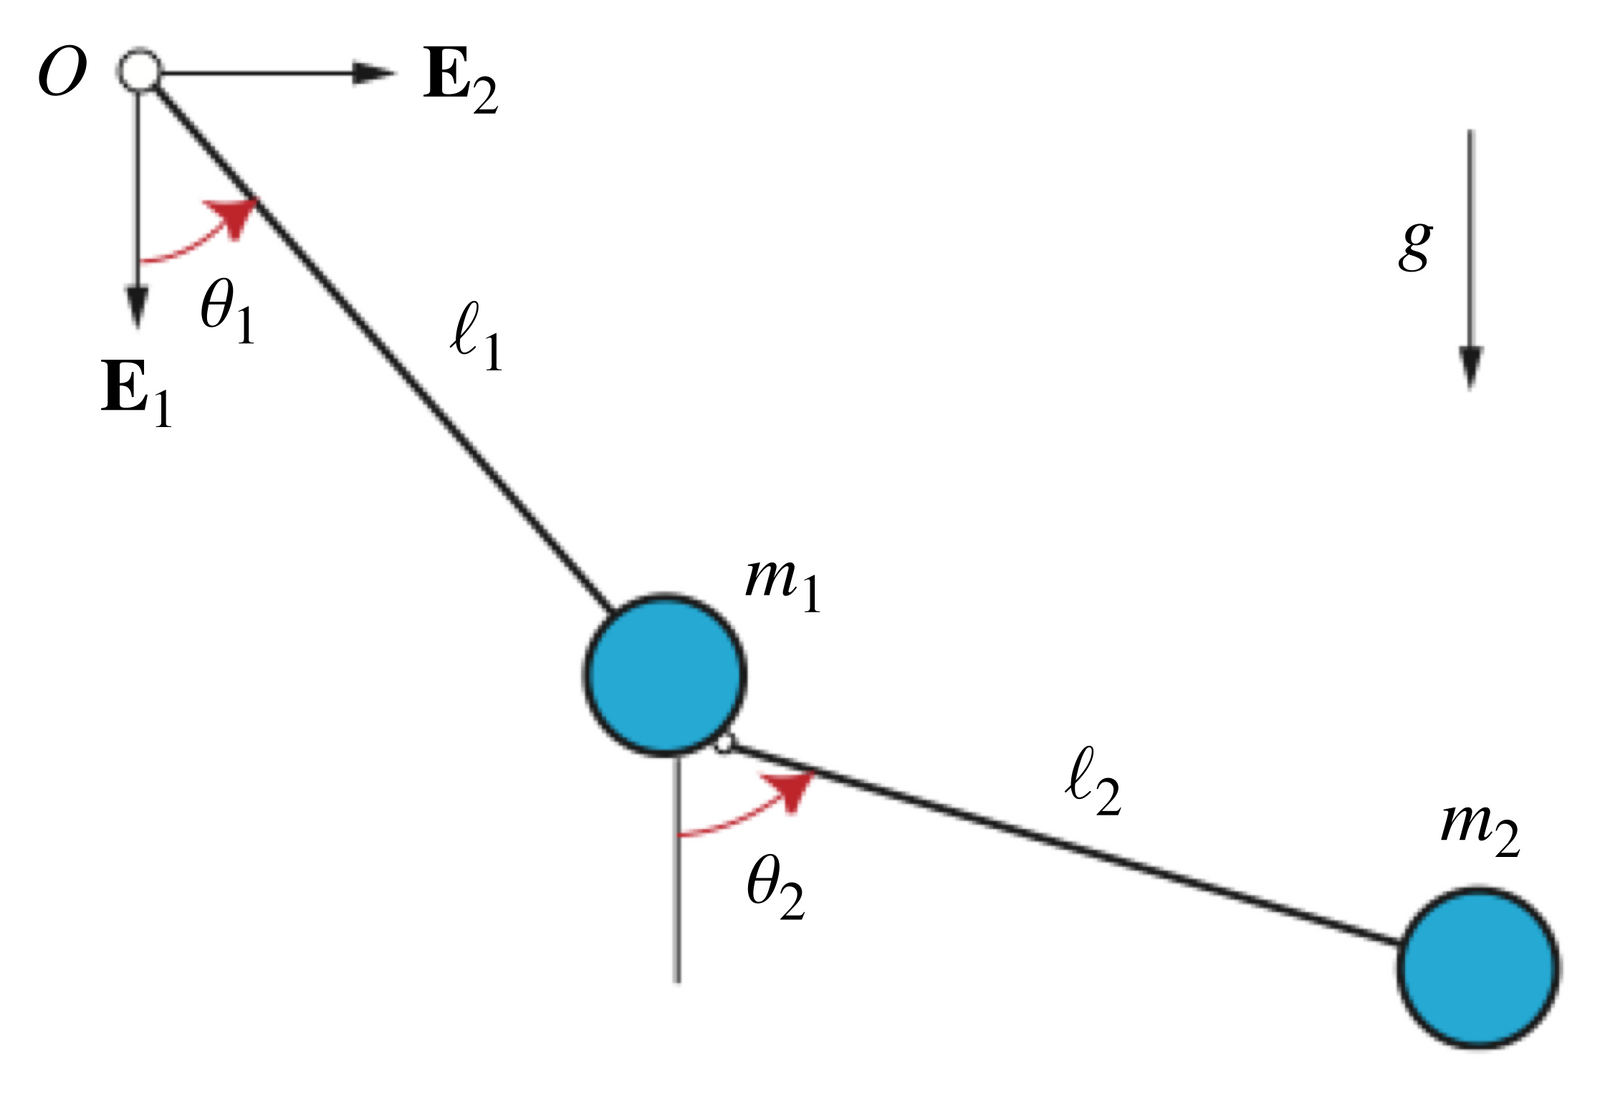
\includegraphics[width=300px]{../assets/double-pendulum.png}
        \end{center}\vspace{2in}
        \question The upper pulley is fixed in position. Both pulleys rotate freely without friction about their axles. 
        Both pulleys are “light” in the sense that their rotational inertias are small and their rotation 
        contributes negligibly to the kinetic energy of the system. The rims of the pulleys are rough, 
        and the ropes do not slip on the pulleys. The gravitational acceleration is $g$. 
        The mass $M$ moves upwards at a rate  $\dot{x}$ with respect to the upper, fixed, pulley, 
        and the smaller pulley moves downwards at the same rate. The mass $m_1$ moves upwards at a rate  
        $\dot{y}$ with respect to the small pulley, and consequently its speed in laboratory space is  
        $\dot{x}-\dot{y}$. The speed of the mass $m_2$ is therefore $\dot{x}+\dot{y}$ in laboratory space. 
        The object is to find  $\ddot{x}$ and  $\ddot{y}$ in terms of  $g$.\\
        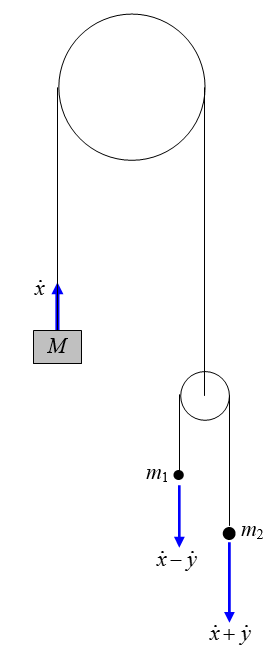
\includegraphics[width=100px]{../assets/figure2.png}
        \question Figure 2 shows a simple pendulum consisting of a string of length $r$ and a bob of mass $m$ that
is attached to a support of mass $M$. The support moves without friction on the horizontal plane. Find what $\ddot{x}$ must be if we want $\ddot{\theta}=0$
        \begin{center}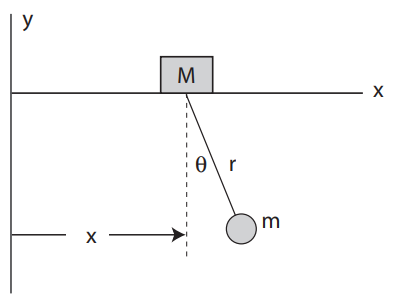
\includegraphics[width=200px]{../assets/figure3.png} \\Figure 2\end{center}
    \end{questions}
\end{document}